% Section content template for individual Educative lessons
% This file contains the actual content for a specific section
% Generated from Educative API section content

% Section: Design of a Distributed Messaging Queue: Part 2
% Section ID: 4953511267139584
% Section Slug: design-of-a-distributed-messaging-queue-part-2
% Generated: 2025-12-07T20:58:24.125402

In the previous lesson, we discussed the responsibilities of front-end servers and metadata services. In this lesson, we'll focus on the main part of the design where the queues and messages are stored: the back-end service.

\subsection{Back-end service}\label{2ckjmvfLLymBMQthoKIFz}
\\
This is the core part of the architecture where major activities take place. When the front-end receives a message, it refers to the metadata service to determine the host where the message needs to be sent. The message is then forwarded to the host and is replicated on the relevant hosts to overcome a possible availability issue. The message replication in a cluster on different hosts can be performed using one of the following two models:

\begin{enumerate}
\item
\protect\phantomsection\label{vGR8wov7tOtVuYxYnC6oC}
\emph{Primary-secondary model}
\item
\protect\phantomsection\label{D0uKdXz1HTDJtO73fnrXa}
\emph{A cluster of independent hosts}
\end{enumerate}
\\
Before delving into the details of these models, let's discuss the two types of cluster managers responsible for queue management: \emph{internal} and \emph{external} cluster managers. The differences between these two cluster managers are shown in the following table.

\textbf{Internal versus External Cluster Managers}

\begin{table}[htbp]
\centering
\small
\adjustbox{max width=\textwidth}{
\begin{tabular}{|p{0.475\textwidth}|p{0.475\textwidth}|}
\hline
\textbf{Internal Cluster Manager} & \textbf{External Cluster Manager} \\
\hline
\hline
It manages the assignment of queues within a cluster. & It manages the assignment of queues across clusters. \\
\hline
It knows about each and every node within a cluster. & It knows about each cluster. However, it doesn't have information on every host that's present inside a cluster. \\
\hline
It listens to the heartbeat from each node. & It monitors the health of each independent cluster. \\
\hline
It manages host failure, instance addition, and removals from the cluster. & It manages and utilizes clusters. \\
\hline
It partitions a queue into several parts and each part gets a primary server. & It may split a queue across several clusters, so that messages for the same queue are equally distributed between several clusters. \\
\hline
\end{tabular}
}
\caption{Internal versus External Cluster Managers}
\end{table}

\subsubsection{Primary-secondary model}\label{2jhuGj8BnWvv79VMZrmhk}
\\
In the \textbf{primary-secondary model}, each node is considered a \textbf{primary host} for a collection of queues. The responsibility of a primary host is to receive requests for a particular queue and be fully responsible for data replication. The request is received by the front-end, which in turn communicates with the metadata service to determine the primary host for the request.
\\
For example, suppose we have two queues with the identities 101 and 102 residing on four different hosts A, B, C, and D. In this example, instance B is the primary host of queue 101 and the secondary hosts where the queue 101 is replicated are A and C. As the front-end receives message requests, it identifies the primary server from the internal cluster manager through the metadata service. The message is retrieved from the primary instance, which is also responsible for deleting the original message upon usage and all of its replicas.
\\
As shown in the following illustration, the internal cluster manager is a component that's responsible for mapping between the primary host, secondary hosts, and queues. Moreover , it also helps in the primary host selection. Therefore, it needs to be reliable, scalable, and performant.

\begin{figure}[htbp]
 \centering
 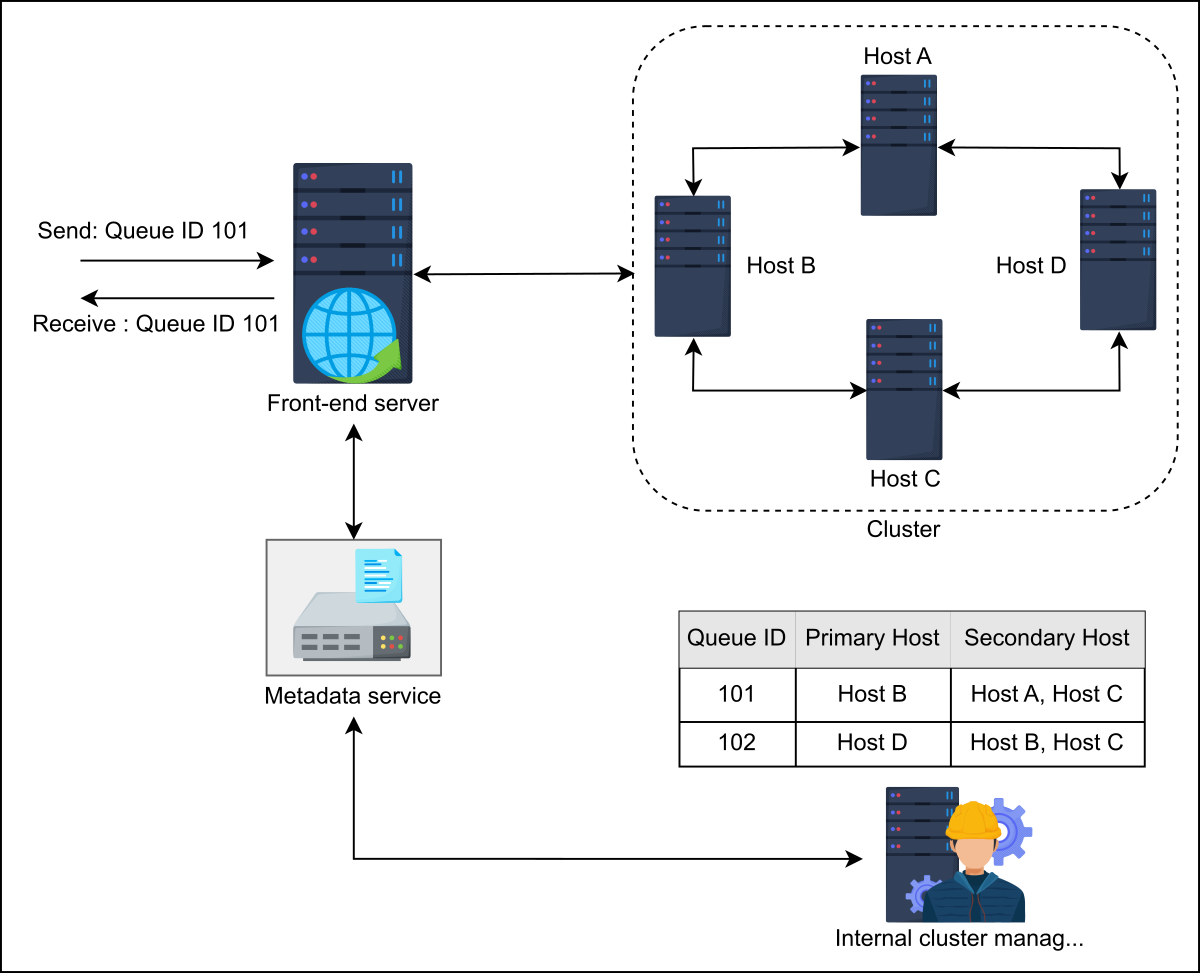
\includegraphics[width=0.5\textwidth]{Images/chapter_17/section_4953511267139584/4978072602673152.png}
 \caption{Primary-secondary model of distributed queue: A request is received for a queue with ID 101, which is served accordingly}
\end{figure}

\subsubsection{A cluster of independent hosts}\label{VkfXUSjp7vuQqLsXRY7Ha}
\\
In the approach involving a \textbf{cluster of independent hosts}, we have several clusters of multiple independent hosts that are distributed across data centers. As the front-end receives a message, it determines the corresponding cluster via the metadata service from the external cluster manager. The message is then forwarded to a random host in the cluster, which replicates the message in other hosts where the queue is stored.

\begin{quote}
\textbf{Quiz:}
\textbf{Question 1:} How does a random host within a cluster replicate data---that is,

messages---in the queues on other hosts within the same cluster?
\textbf{Answer:} Each host consists of mapping between the queues and the hosts within a cluster, making the replication easier. Assume that we have a cluster,

say Y, having hosts A, B, and C. This cluster has two queues with IDs 101 and 103 stored on different hosts, as shown in the following table.
This table is stored on each host within the cluster Y. When a random host receives a message, say host C, for a queue having ID 103, host C replicates this message on the other hosts where the queue 103 is stored, i.e., Node A and Node B.

\end{quote}

The same process is applied to receive message requests from the consumer. Similar to the first approach, the randomly selected host is responsible for message delivery and cleanup upon a successful processing of the message.
\\
Furthermore, another component called an \textbf{external cluster manager} is introduced, which is accountable for maintaining the mapping between queues and clusters, as shown in the following figure. The external cluster manager is also responsible for queue management and cluster assignment to a particular queue.
\\
The following figure illustrates the cluster of independent hosts. There are two clusters, A and B, which consist of several nodes. The external cluster manager has the mapping table between queues and their corresponding cluster. Whenever a front-end receives a request for a queue, it determines the corresponding cluster for the queue and forwards the request to the cluster where the queue resides. The nodes within that cluster are responsible for storing and sending messages accordingly.

\begin{figure}[htbp]
 \centering
 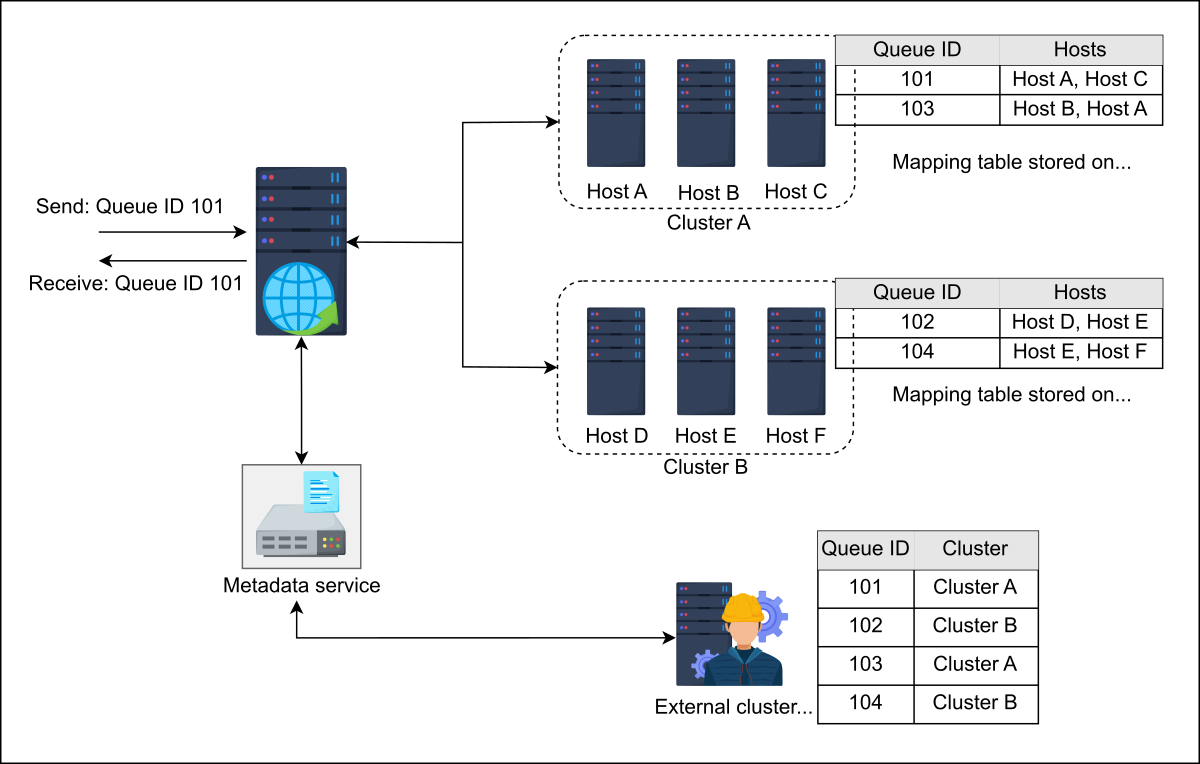
\includegraphics[width=0.5\textwidth]{Images/chapter_17/section_4953511267139584/6009555883786240.png}
 \caption{A cluster of independent hosts that consist of distributed queues}
\end{figure}

\begin{quote}
\textbf{Quiz:}
\textbf{Question 1:} How is message replication handled in distributed queue systems?
\textbf{Answer:} There are two ways to replicate messages in a queue residing on multiple hosts. 1. Synchronous replication 2. Asynchronous replication In synchronous replication, the primary host is responsible for replicating the message in all the relevant queues on other hosts. After acknowledgment from secondary hosts, the primary host then notifies the client regarding the reception of messages. In this approach, messages remain consistent in all queue replicas; however, it costs extra delay in communication and causes partial to no availability while an election is in progress to promote a secondary as a primary. In asynchronous replication, once the primary host receives the messages, it acknowledges the client and, in the next step, starts replicating the message to other hosts. This approach has other problems, such as replication lag and consistency issues. Based on the needs of an application, we can pick one or the other.
\end{quote}

We have completed the design of a distributed messaging queue and discussed the two models for organizing the back-end server. We also described the management process of queues and how messages are processed at the back-end. Furthermore , we discussed how back-end servers are managed through different cluster managers.
\\
In the next lesson, we'll discuss how our system fulfills the functional and non-functional requirements that were described earlier in the chapter.

% End of section content